%% Thresholds That Travel -- anonymous submission, USENIX Security (second template copy).
%% Body text, tables, figures and numbers are identical to latex/main.tex (the ACM sigconf
%% version); only the class, front matter and bibliography style differ.
%% Anonymization: no author block, no ORCID, no repository links, no DOIs of the authors' own
%% artifacts; the artifact is an anonymous.4open.science placeholder (see the TODOs).
%% Third-party dataset DOIs (HyGrid-ICS, BATADAL, voraus-AD) are retained deliberately.
%%
%% To use the official template, drop usenix-2020-09.sty (from the USENIX Security author
%% resources) next to this file; it is picked up automatically below. Without it, the fallback
%% geometry reproduces the same page metrics (letter, two columns, 10pt).
\documentclass[letterpaper,twocolumn,10pt]{article}

\IfFileExists{usenix-2020-09.sty}{\usepackage{usenix-2020-09}}{%
  \usepackage[letterpaper,top=1in,bottom=1in,left=0.75in,right=0.75in,columnsep=0.33in]{geometry}
  \usepackage{times}
  \setlength{\parindent}{9pt}
}

\usepackage{booktabs}
\usepackage{array}
\usepackage{graphicx}
\usepackage{url}
\usepackage[hidelinks]{hyperref}
\usepackage{cite}

\title{\Large \bf Thresholds That Travel: Adaptive Alarm Thresholds Let Attacks Through in
  ICS Anomaly Detection}

%% Author block removed for anonymous review.
\author{}
\date{}

\begin{document}

\maketitle
\thispagestyle{empty}
\pagestyle{plain}

\begin{abstract}
Anomaly detectors for industrial control systems (ICS) raise an alarm when a score crosses a
threshold. The threshold is calibrated on clean data and must then hold a false-alarm budget
for months, so deployments often let it adapt: they recalibrate it daily, track a running
quantile, or refit an extreme-value tail as data arrive. We show that whatever an adaptive
threshold learns from, an attacker can feed it, and that real attacks feed some of these rules
without any adversarial effort.

We ran a pre-registered study on three datasets that no earlier analysis in our pipeline had
opened (HAI 20.07, HyGrid-ICS and voraus-AD), with a world-model residual monitor and eleven
threshold rules. On HAI 20.07's 38 attacks the frozen threshold detected 36 at 2.23 false-alarm
episodes per day; a symmetric quantile tracker detected 20 (difference $-0.42$, 95\% interval
$[-0.58, -0.26]$) because earlier attacks had raised its threshold a median 12.9 times above
calibration. Daily recalibration and a ten times slower tracker also lost recall, and the same
loss appeared on HyGrid-ICS and voraus-AD, on three earlier HAI releases, and with a second,
model-free score. On attack-free development data, twelve two-minute nuisance alarms a day
blinded every rule that learns from exceedances to a later, just-detectable setpoint attack; on
the registered HAI 20.07 stream the real attacks had already done the same before any pulse
arrived.

Streaming extreme-value thresholds (SPOT and DSPOT) refuse to learn from alarms and escaped this
natural poisoning on the HAI data, but a closed-loop attacker who holds the score just under the
current threshold drove their thresholds upward without raising one alarm and blinded them within
an hour. A second registered study on the BATADAL water network replicated the tracker's loss
(6 of 14 attacks against 14 for the frozen threshold) and showed that slow, days-long attacks also
inflate SPOT and DSPOT. Its registered primary rule nevertheless failed: the third hypothesis,
that a closed-loop attacker blinds DSPOT, could not be tested because real attacks had already
blinded DSPOT in all ten controls. Across seven datasets, a threshold that only tightens itself
matched the frozen threshold's recall every time, while every rule that can raise its own
threshold lost recall on at least one. We argue that an alarm threshold may tighten itself but
should loosen only with operator approval, and we release the registrations, ledger and code.
\end{abstract}

\section{Introduction}

A process-monitoring anomaly detector has two parts: a score that grows when the plant behaves
unlike its normal operation, and a threshold that turns the score into alarms. Most of the
research effort goes into the score. The threshold is usually set once, on held-out normal data,
to meet a false-alarm budget, and then expected to hold that budget on a plant that drifts:
sensors age, seasons change load, and operators retune loops. When it does not hold, the standard
remedies adapt the threshold online. Daily recalibration re-estimates a quantile on the last day
of data. Online quantile tracking, the mechanism behind adaptive conformal
inference~\cite{gibbs2021aci}, nudges the threshold up after every exceedance and down otherwise.
Streaming peaks-over-threshold methods (SPOT and DSPOT~\cite{siffer2017spot}) refit a generalised
Pareto tail as new values arrive, and the nonparametric dynamic threshold of
Telemanom~\cite{hundman2018telemanom} recomputes its level on a trailing window.

Each of these rules learns from part of its input. Trackers and recalibration learn from the
values that exceed the threshold. SPOT and DSPOT discard values above their alarm level but learn
from values between a base level and the alarm level. A frozen threshold learns from nothing after
calibration. We call the part of the score range a rule learns from its \emph{learning region},
and the question of this paper is what happens when an attack, or an attacker, lands in it.

The answer depends on the region, and none of the adaptive rules we tested is safe:

\begin{itemize}
\item \textbf{Rules that learn from exceedances are poisoned by real attacks.} An attack is a long
  exceedance, so a tracker raises its threshold during the attack and stays high afterwards. The
  next attack then arrives under an inflated threshold. On fresh HAI 20.07 data the tracker missed
  18 of 38 attacks, 16 of them attacks the frozen threshold caught. No adversarial planning is
  needed; the attacks in the recording did it.
\item \textbf{The same rules can be poisoned on purpose and loudly.} Twelve two-minute pulses a
  day, the kind of nuisance alarm operators learn to acknowledge, raised these thresholds enough to
  hide a later attack that a frozen threshold caught every time (attack-free development data).
\item \textbf{Rules that refuse to learn from alarms can be poisoned silently.} An attacker who
  reads the current SPOT or DSPOT threshold and holds the score just under it feeds every sample
  into the fitted tail. The tail extends, the threshold rises, the attacker follows it up, and no
  alarm is ever raised.
\end{itemize}

A threshold that only tightens automatically, and loosens only when an operator approves, resisted
all three. Its cost is extra false alarms when the plant drifts upward.

\paragraph{Method}
The main study was registered before any test file, label or attack schedule of its three datasets
was read. A ledger records every access to recorded attack data, the analysis harness refuses to
run if any frozen source file changed after registration, and it computes the registered gates
itself. The rules and the attack designs came from development on three earlier HAI releases whose
attacks had already been used; we report how the claim changed during development, including two
hypotheses we dropped. Extensions run after the registered finals are labelled exploratory.

\paragraph{Contributions}
\begin{enumerate}
\item A registered comparison of eleven threshold rules on three never-opened datasets from three
  systems (a hardware-in-the-loop ICS testbed, a simulated hybrid power grid, and an industrial
  robot), with real-event recall, false-alarm rates and threshold trajectories (Section~\ref{sec:registered}).
\item Evidence that exceedance-learning thresholds lose recall on real attacks because earlier
  attacks inflate them, on seven datasets and two score families, with the mechanism visible in
  which attacks are missed, and a registered replication on the BATADAL water network
  (Sections~\ref{sec:registered} and~\ref{sec:regions}).
\item A learning-region analysis of adaptive thresholds with a matching attack for each class:
  supra-threshold pulse campaigns for exceedance learners and a closed-loop frog-boiling attack for
  extreme-value learners, including how the latter depends on the tail estimator
  (Section~\ref{sec:regions}).
\item A design rule, supported by these results, for deployed detectors: thresholds may tighten
  themselves; loosening needs a human (Section~\ref{sec:design}).
\item The registration, access ledger, harness and verifier, in the anonymized artifact at
  \url{https://anonymous.4open.science/...}.
  % TODO: replace with the anonymous.4open.science URL of the anonymized artifact before submission.
\end{enumerate}

\section{Background and related work}

\paragraph{ICS anomaly detection}
Process-level detectors learn normal behaviour from sensor and actuator traces and flag deviations:
residuals of a predictive model, reconstruction errors of an autoencoder, or statistical bounds.
Public testbed recordings with labelled attacks (SWaT~\cite{goh2016swat}, WADI~\cite{ahmed2017wadi},
BATADAL~\cite{taormina2018batadal}, and the HAI releases~\cite{shin2020hai} for HAI 1.0 (20.07);
later releases are documented in the dataset repository) are the usual benchmarks. Evaluations
typically fix one threshold per detector, chosen on clean data or, less defensibly, on the test
labels. Wu and Keogh~\cite{wu2023benchmarks} list further benchmark pitfalls.

\paragraph{Threshold rules}
Static thresholds come from a quantile or a false-alarm budget on clean data. Adaptive variants
recalibrate on a trailing window, track a target exceedance rate online~\cite{gibbs2021aci}, fit an
extreme-value tail and update it per observation (SPOT, and DSPOT for drifting
streams~\cite{siffer2017spot}), or recompute a level on a trailing window of smoothed
errors~\cite{hundman2018telemanom}. Alarm-management practice in process plants treats nuisance and
chattering alarms as a condition to eliminate, with explicit alarm-rate
targets~\cite{isa182}; operators who acknowledge such alarms without investigating them are the
failure mode our pulse campaigns exploit.

\paragraph{Poisoning of anomaly detectors}
Rubinstein et al.~\cite{rubinstein2009antidote} showed that slowly shifted traffic (``boiling
frog'' poisoning) can stop a PCA-based network anomaly detector from flagging a later attack. Kloft
and Laskov~\cite{kloft2010online} analysed poisoning of online centroid detectors. Chan-Tin
et al.~\cite{chantin2009frog} described the frog-boiling attack on outlier rejection in network
coordinate systems, where every update stays within the rejection threshold while the system
drifts. In ICS, Kravchik and Shabtai~\cite{kravchik2020frog} found that autoencoder detectors
retrained online on SWaT resisted their poisoning attacks, and Erba et al.~\cite{erba2020concealment}
concealed attacks from reconstruction-based detectors by manipulating sensor readings.
Hong~\cite{hong2026boiling} studied gradual drift against world-model monitors in simulation,
without attacks or adaptive thresholds. These works target the model or the score. We target the
threshold rule and show that it can fail even when the model resists poisoning.

\paragraph{Distribution shift and calibration}
Adaptive conformal inference keeps a long-run miscoverage rate under arbitrary shift, a guarantee
about the rate of exceedances. That guarantee holds whether the exceedances come from benign drift
or from attacks, which is the property we exploit in Section~\ref{sec:regions}.

\section{Threat model and learning regions}
\label{sec:threat}

\paragraph{System}
A monitor computes a score $s_t$ from plant telemetry and raises an alarm when $s_t > \tau_t$. The
rule that sets $\tau_t$ is calibrated once on clean data to a false-alarm budget and then runs
online. Operators acknowledge alarms; persistent nuisance alarms are acknowledged without
investigation.

\paragraph{Learning region}
For a rule $R$, the learning region $L(R, \tau_t)$ is the set of score values that change $R$'s
future thresholds. Table~\ref{tab:regions} gives the rules we study.

\begin{table*}[t]
\caption{Update and learning region of each threshold rule.}
\label{tab:regions}
\begin{tabular}{@{}lll@{}}
\toprule
Rule & Update & Learning region \\
\midrule
frozen, static margin & none & empty \\
symmetric tracker $q_{t+1} = q_t + \eta(\mathbf{1}[s_t > q_t] - p)$ & up on exceedance, down otherwise & all values; upward moves only from $s_t > \tau_t$ \\
daily recalibration & $(1 - p)$ quantile of the last day & the top $p$ of each day, whatever its source \\
SPOT & adds $s_t - t$ to the tail fit when $t < s_t \le z_q$ & the band $(t, \tau_t]$ \\
DSPOT & as SPOT on $s_t$ minus a moving mean of non-alarm values & the band, plus every non-alarm value through the mean \\
tighten-only & $\min(\text{ceiling}, \text{tracker})$; the ceiling rises only through a permit & downward only, unless a permit fires \\
\bottomrule
\end{tabular}
\end{table*}

\begin{figure*}[t]
\centering
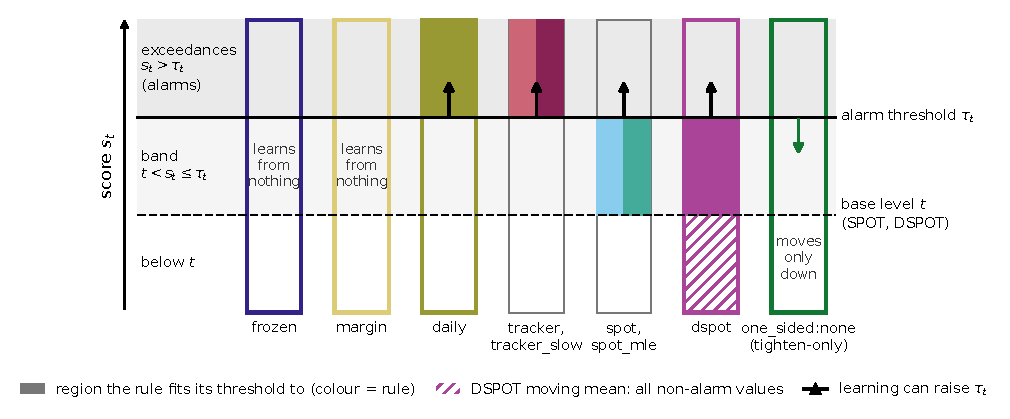
\includegraphics[width=\textwidth]{figures/fig1_learning_regions.pdf}
\caption{Learning regions of the threshold rules (schematic). The alarm threshold $\tau_t$ and, for
SPOT and DSPOT, the base level $t$ below it split the score range into exceedances ($s_t > \tau_t$),
the band ($t < s_t \le \tau_t$) and values below $t$. A filled column segment marks the region a rule
fits its threshold to; DSPOT's moving mean also absorbs every non-alarm value (hatched). Daily
recalibration and the trackers learn from exceedances, so the attacks they are meant to detect raise
their thresholds; frozen and the static margin learn from nothing; one\_sided:none can only move
downward. Data status: schematic with no data, so the registered / exploratory / post-hoc label does
not apply; the rule behaviour follows Table~\ref{tab:regions}.}
\label{fig:regions}
\end{figure*}

A rule can loosen (raise $\tau_t$) only through values in the part of its learning region that
pushes upward. That gives three attacker classes, from weakest to strongest:

\begin{itemize}
\item \textbf{A0, no attacker.} Real attacks are themselves exceedances. A rule whose upward
  learning region includes exceedances is poisoned by the attacks it is meant to detect.
\item \textbf{A1, open-loop injection.} The attacker can perturb one control loop (setpoints or
  sensor readings) without seeing the monitor. Supra-threshold pulses land in the exceedance
  region; sub-alarm pulses land in the band.
\item \textbf{A2, closed-loop.} The attacker can read $\tau_t$ (white-box, or by probing) and shape
  the score. Holding $s_t$ at $0.97\,\tau_t$ places every sample at the top of the band with no
  alarm. We evaluate A2 at the score level, an upper bound on what a physical attacker can do, and
  through noise spoofed onto three sensor readings of one loop, scored by the real monitor.
\end{itemize}

The attacker's goal is a terminal attack that the frozen threshold would detect but the adapted
threshold does not.

\section{Monitor, rules and data}
\label{sec:setup}

\paragraph{Monitor}
D1 is the world-model residual monitor of earlier registered studies on HAI [anonymized]: an
action-conditioned ridge regression with LightGBM residual corrections (60 trees, history 3)
predicts each sensor one and five steps ahead; the score is the mean of the three largest
standardised absolute residuals at each horizon, summed and smoothed over 60\,s. D0 is a model-free
control: the mean of the three largest standardised first differences. Both are calibrated on the
most recent 20\% of normal training data: to 2 false-alarm episodes per day on the 1\,Hz stream
datasets (episodes merged across 60\,s gaps), to a per-sample false-alarm target of 0.05 on
voraus-AD, and to one false-alarm episode per week on BATADAL (episodes merged across 1\,h).

\paragraph{Rules}
frozen ($\tau_0$ at the budget); margin ($\tau_0 + 0.25 \times$ the spread between the calibration
99.9th percentile and median); daily (trailing-day quantile at the calibration exceedance rate $p$);
tracker ($\eta = 0.01 \times$ spread on the stream datasets, $0.05 \times$ spread on voraus-AD) and
tracker\_slow ($\eta / 10$, the best false-alarm adherence among trackers in development);
tighten-only with four automatic permits and an oracle permit that simulates an operator who refuses
to loosen while an event is under way: eleven rules in all. On voraus-AD the spread is the
calibration 99th percentile minus the median and daily recalibration happens every 50 samples. The
streaming extreme-value rules (SPOT and DSPOT, with method-of-moments and maximum-likelihood tail
fits~\cite{hosking1987gpd, siffer2017spot}) were not part of the tt1 registration: they enter in
Section~\ref{sec:regions} as exploratory and post-hoc analyses and are registered only in the
BATADAL replication (tt1b).

\begin{table*}[t]
\caption{Datasets. Event counts are the labelled events of each final split.}
\label{tab:data}
\begin{tabular}{@{}lllll@{}}
\toprule
Dataset & System & Training data & Final data & Events \\
\midrule
HAI 20.07 (primary) & HIL testbed (boiler, turbine, water treatment) & 547,624\,s normal, 31 sensors, 20 actions & test1 + test2, 5.15 days & 38 attacks \\
HyGrid-ICS & simulated hybrid grid SCADA, 5\,Hz to 1\,Hz & 9.6\,h (label-blind first 40\%) & 14.5\,h & 91 attacks \\
voraus-AD & industrial robot, 100\,Hz to 10\,Hz & 948 normal samples & 1174 samples & 755 anomalous samples \\
HAI 21.03, 22.04, 23.05 (development) & HIL testbed & normal training data & spent test files & 50, 58, 52 attacks \\
BATADAL (registered replication) & water distribution network, 15\,min & 384 days normal & two test files, 260 days & 14 attacks \\
\bottomrule
\end{tabular}
\end{table*}

\paragraph{Registration}
The protocol fixed the monitor, splits, rules, injection designs, gates and seeds; the harness
recorded one ledger entry per dataset before reading a test array, refused to run if a frozen file's
SHA-256 differed from the registration, and computed the gates from its own output. A verifier
checks that each access followed the registration commit, that each dataset was opened once, and
that the stored gates match a recomputation (27 of 27 checks pass).

\section{How the hypothesis changed during development}
\label{sec:development}

All development used normal training data and the already-opened attack files of HAI 21.03, 22.04
and 23.05. We report it because the registered claim differs from the one we set out to test.

\begin{enumerate}
\item \emph{Tighten-only with automatic loosening.} Our starting design let a threshold tighten
  itself and loosen only through a statistical permit. A slow sub-threshold drift (``boiling frog''
  in the style of Rubinstein et al.) did not poison any rule: the world model absorbed the drift.
  Supra-threshold pulses did inflate the trackers, but every automatic permit we tried either opened
  under the pulses (spread permit: 3 of 30 terminal attacks caught in development round r3, 5 of 30
  in round r4) or failed to follow benign drift (shift permit).
\item \emph{Static safety margin.} A margin at half the calibration exceedance rate cut the
  false-alarm rate on pseudo-deployment splits without always reaching the budget (HAI 20.07
  development: 3.79 episodes per day against 4.42 for frozen, budget 2), and cost 4 to 10 points of
  recall on the spent attacks (interval lower bounds down to $-0.17$), so we registered a smaller
  margin and made it secondary.
\item \emph{Frozen versus adaptive.} On the spent attacks the frozen threshold held the budget on
  all three real test periods (0.66, 1.48 and 1.27 episodes per day), while the tracker lost 22, 31
  and 37 points of recall with intervals entirely below zero. This became the registered primary.
\end{enumerate}

\section{Registered results}
\label{sec:registered}

\subsection{Primary: HAI 20.07}

\begin{table*}[t]
\caption{Registered gates of tt1 on HAI 20.07. Data status: \textbf{registered}.}
\label{tab:gates}
\begin{tabular}{@{}p{0.04\textwidth}p{0.55\textwidth}p{0.33\textwidth}@{}}
\toprule
Gate & Registered test & Result \\
\midrule
G1 & after a pulse campaign ($12 \times 120$\,s per day at twice the terminal magnitude), daily, tracker and tracker\_slow detect the terminal step in at most (frozen $-$ 0.5) of placements; frozen at least 0.8 & frozen 10/10, each adaptive rule 0/10: pass \\
G2 & recall(tracker) $-$ recall(frozen) on the real attacks, 95\% paired event bootstrap upper bound below 0 & 0.526 vs 0.947, $-0.42$ $[-0.58, -0.26]$: pass \\
G3 & frozen false-alarm episodes per day on unlabelled test time at most 4 & 2.23: pass (above the 2.0 budget) \\
\bottomrule
\end{tabular}
\end{table*}

False-alarm episodes per day are counted over the 4.94 days of unlabelled time inside the 5.15-day
test streams. G1 passes as registered, but on this stream the pulses were not needed: the adaptive
rules also missed the terminal step in the control runs, because the test stream's real attacks had
already raised their thresholds 7 to 26 times above $\tau_0$. The pulse effect in isolation comes
from development on attack-free normal data (frozen 30/30; daily 4/30, control 21/30; tracker 1/30,
control 23/30; tracker\_slow 3/30, control 25/30).

\subsection{Real attacks inflate adaptive thresholds}
\label{sec:inflate}

\begin{table*}[t]
\caption{Event recall and the paired difference against the frozen threshold (95\% paired event
bootstrap) on the D1 score. Data status: \textbf{registered} (tt1).}
\label{tab:recall}
\begin{tabular}{@{}lccccc@{}}
\toprule
Dataset (events) & frozen & daily & tracker & tracker\_slow & tighten-only \\
\midrule
HAI 20.07 (38 attacks) & 0.947 & 0.474 $[-0.63, -0.32]$ & 0.526 $[-0.58, -0.26]$ & 0.711 $[-0.37, -0.11]$ & 0.947 \\
HyGrid-ICS (91 attacks) & 0.297 & 0.297 & 0.154 $[-0.22, -0.08]$ & 0.165 $[-0.21, -0.07]$ & 0.297 \\
voraus-AD (755 anomalous samples) & 0.334 & 0.148 $[-0.21, -0.16]$ & 0.082 $[-0.28, -0.22]$ & 0.213 $[-0.14, -0.10]$ & 0.334 \\
\bottomrule
\end{tabular}
\end{table*}

At HAI 20.07 attack onsets the median threshold stood at 25.6 $\tau_0$ for daily recalibration, 12.9
for the tracker and 6.4 for the slow tracker. HyGrid's daily rule equals frozen because its 14.5\,h
final never completes a day.

\begin{figure}[t]
\centering
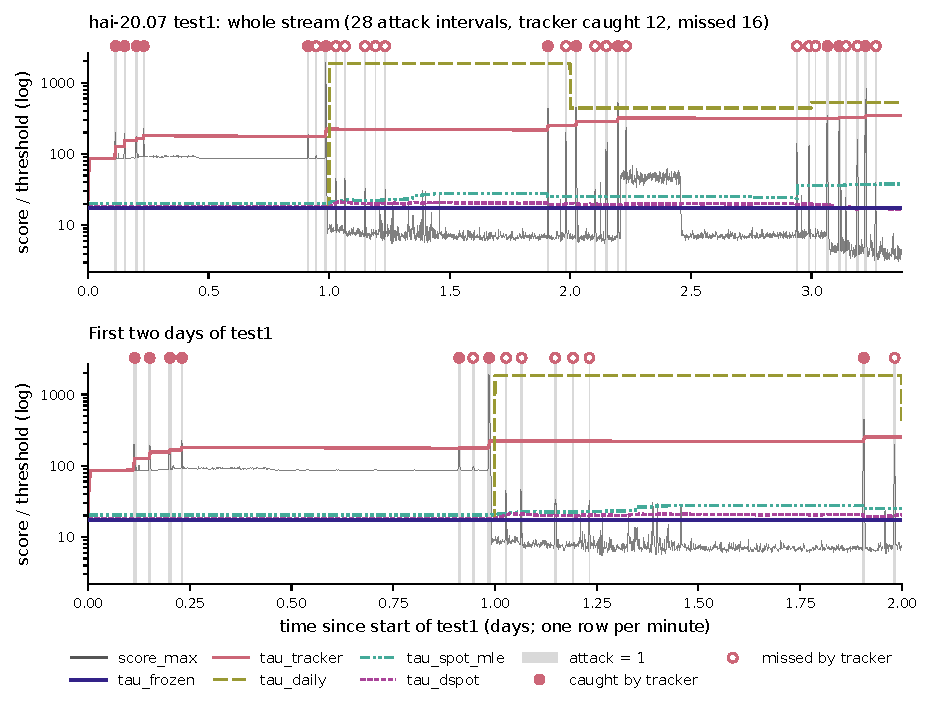
\includegraphics[width=\columnwidth]{figures/fig2_trajectories_hai2007.pdf}
\caption{Threshold trajectories on the HAI 20.07 test1 stream (4,860 minutes). Grey: the D1 score
score\_max. Coloured: the frozen, tracker, daily, spot\_mle and dspot thresholds, log scale. Grey
shading marks attack-labelled minutes; each marker above the panel is one attack interval, filled if
the tracker caught it. test1 holds 28 of the 38 attacks; the tracker caught 12. Early attacks raise
the tracker and daily thresholds far above frozen ($\tau_0 = 17.26$), and later attacks arrive under
the inflated thresholds. Data status: \textbf{post-hoc analysis}; the trajectories were computed
after the registered finals. The recomputed calibration threshold equals the registered one exactly.
Over test1 and test2 the traces give frozen 36/38 and tracker 20/38 (registered tt1) and spot\_mle
35/38 and dspot 36/38 (post-hoc: SPOT and DSPOT were not in the tt1 registration). test2 is not
drawn; test1 has no missing values.}
\label{fig:hai}
\end{figure}

\begin{figure*}[t]
\centering
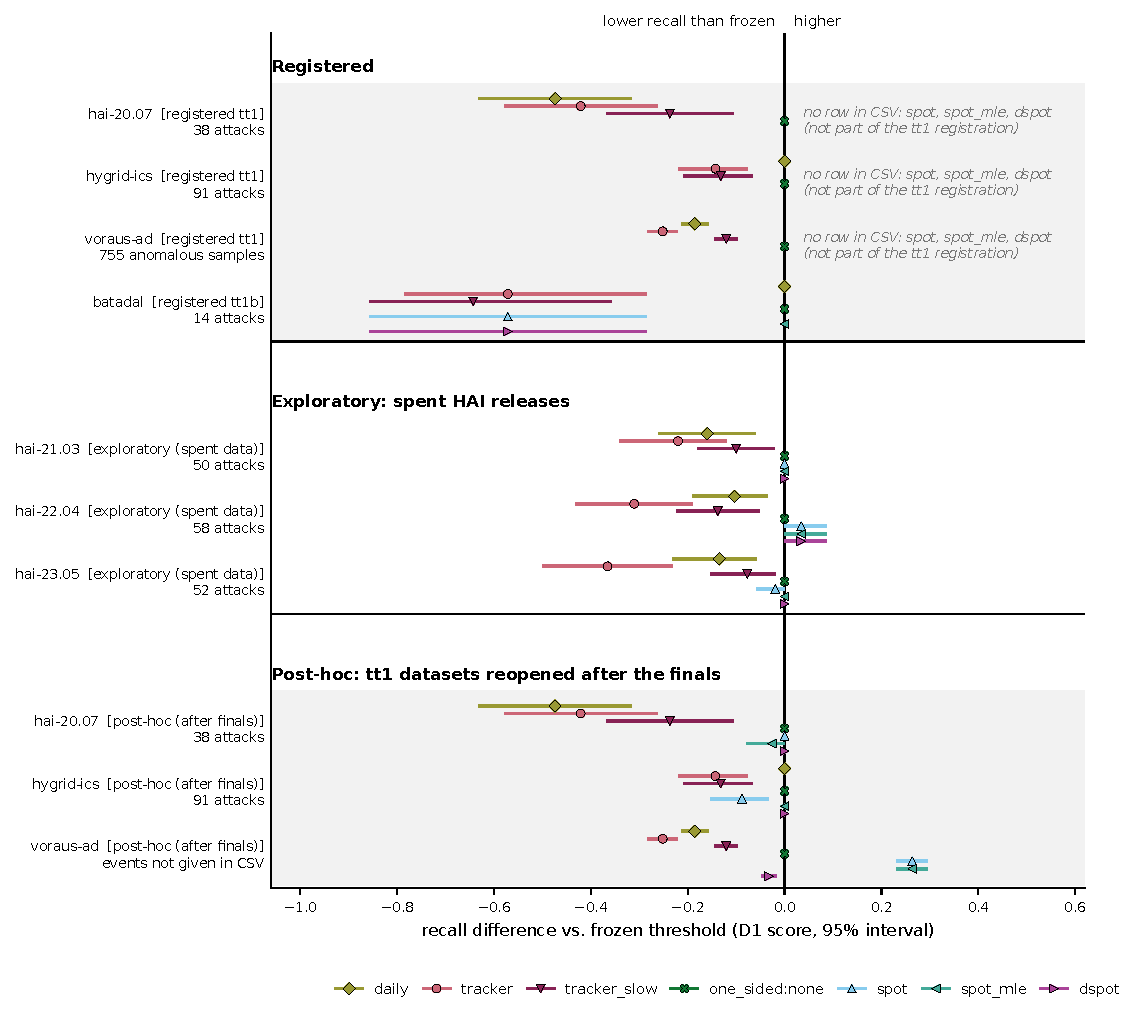
\includegraphics[width=0.92\textwidth]{figures/fig4_recall_forest.pdf}
\caption{Paired difference in event recall between each adaptive rule and the frozen threshold on
D1, with 95\% intervals. Values left of 0 mean lower recall than frozen. Three blocks, each row
labelled with its data status: (1) \textbf{registered} results from tt1 (hai-20.07, hygrid-ics,
voraus-ad) and tt1b (batadal); (2) \textbf{exploratory} development results on the spent HAI
releases; (3) \textbf{post-hoc} results on the tt1 datasets, reopened after the finals. spot,
spot\_mle and dspot have no rows for the registered tt1 datasets because those rules were not part
of the tt1 registration; the gaps are labelled and the post-hoc block supplies the comparisons.
one\_sided:none equals frozen (0 $[0, 0]$) in every block. The positive spot and spot\_mle values
for voraus-ad (post-hoc) are not a gain: with 190 calibration samples SPOT ran at a per-sample
false-positive rate of 0.32 against the 0.05 target (Section~\ref{sec:evt}).}
\label{fig:forest}
\end{figure*}

\subsection{False alarms}

\begin{table}[t]
\caption{False alarms. Data status: \textbf{registered} (tt1).}
\label{tab:falsealarms}
\small
\begin{tabular}{@{}p{0.30\columnwidth}ccccc@{}}
\toprule
Dataset & frozen & margin & daily & tracker & tracker\_slow \\
\midrule
HAI 20.07 (episodes/day) & 2.23 & 2.23 & 0.20 & 1.01 & 2.23 \\
HyGrid-ICS (episodes/day, 2.5\,h unlabelled) & 19.2 & 0.0 & 19.2 & 19.2 & 19.2 \\
voraus-AD (per-sample FPR, target 0.05) & 0.081 & 0.033 & 0.086 & 0.012 & 0.014 \\
\bottomrule
\end{tabular}
\end{table}

Where an adaptive rule raised fewer false alarms than frozen, it bought them with the recall losses
of Section~\ref{sec:inflate}. The one rule that cut false alarms at no recall cost here, the static
margin on HyGrid-ICS (0.0 against 19.2 per day at identical recall), does not adapt. The margin
matched frozen recall on HAI 20.07 and held voraus-AD's target at a cost of 12 points of recall
there.

\section{Learning regions under attack (exploratory)}
\label{sec:regions}

The analyses in this section were not registered. They use the spent HAI releases for development
and reopen the three tt1 datasets after their finals; every access is in the ledger.

\subsection{Extreme-value thresholds escape natural poisoning on the HAI data}
\label{sec:evt}

\begin{table*}[t]
\caption{Event recall of the extreme-value rules. Data status: \textbf{exploratory} on the spent
releases, \textbf{post-hoc} on HAI 20.07.}
\label{tab:evt}
\begin{tabular}{@{}lccccc@{}}
\toprule
Data & frozen & tracker & SPOT (moments) & SPOT (MLE) & DSPOT \\
\midrule
HAI 21.03 / 22.04 / 23.05 & 1.00 / 0.76 / 0.60 & 0.78 / 0.45 / 0.23 & 1.00 / 0.79 / 0.58 & 1.00 / 0.79 / 0.60 & 1.00 / 0.79 / 0.60 \\
HAI 20.07 (post-hoc) & 0.947 & 0.526 & 0.947 & 0.921 $[-0.08, 0.00]$ & 0.947 \\
\bottomrule
\end{tabular}
\end{table*}

The exceptions: on HyGrid-ICS the moments SPOT lost 9 points ($[-0.15, -0.03]$); on voraus-AD, 190
calibration samples leave about four tail points above SPOT's base level (the calibration 98th
percentile), and SPOT ran at 32\% false positives against a 5\% target.

\subsection{The effect does not depend on the score}

With D0 the tracker lost recall on every dataset where it was measured: $[-0.38, -0.14]$,
$[-0.21, -0.05]$ and $[-0.19, -0.02]$ on the spent releases, $[-0.32, -0.08]$ on HAI 20.07 and
$[-0.12, -0.02]$ on HyGrid-ICS.

\subsection{Mechanism: attacks that follow attacks}

The tracker's misses concentrate on attacks that start within 6\,h of the previous attack's end. D1
recall on close versus isolated attacks was 0.75 / 1.00, 0.41 / 1.00 and 0.20 / 0.67 on the spent
releases and 0.48 / 0.71 on HAI 20.07 (31 close, 7 isolated). The frozen threshold also detected
close attacks less often on two releases, so part of the gap reflects harder attacks; the tracker's
gap is larger on every release.

\subsection{Loud poisoning: pulse campaigns}
\label{sec:pulses}

Normal data of the spent releases, 30 placements; the terminal step is the smallest setpoint step
the frozen threshold detects on the clean stream.

\begin{table*}[t]
\caption{Terminal attacks caught after a pulse campaign (control in parentheses). Data status:
\textbf{exploratory} (normal data of the spent releases).}
\label{tab:pulses}
\begin{tabular}{@{}lcccccc@{}}
\toprule
Campaign & frozen & daily & tracker & tracker\_slow & SPOT & DSPOT \\
\midrule
$12 \times 120$\,s supra-threshold pulses per day & 30/30 (30/30) & 4/30 (21/30) & 1/30 (23/30) & 3/30 (25/30) & 29/30 (30/30) & 23/30 (25/30) \\
$24 \times 300$\,s sub-alarm pulses per day, open loop & 30/30 & 23/30 (23/30) & 19/30 (21/30) & 23/30 & 29/30 & 22/30 (24/30) \\
\bottomrule
\end{tabular}
\end{table*}

Open-loop sub-alarm pulses did not poison SPOT: its threshold fell (0.82 to 0.98 $\tau_0$), and many
pulses crossed SPOT's own alarm level and were refused.

\begin{figure}[t]
\centering
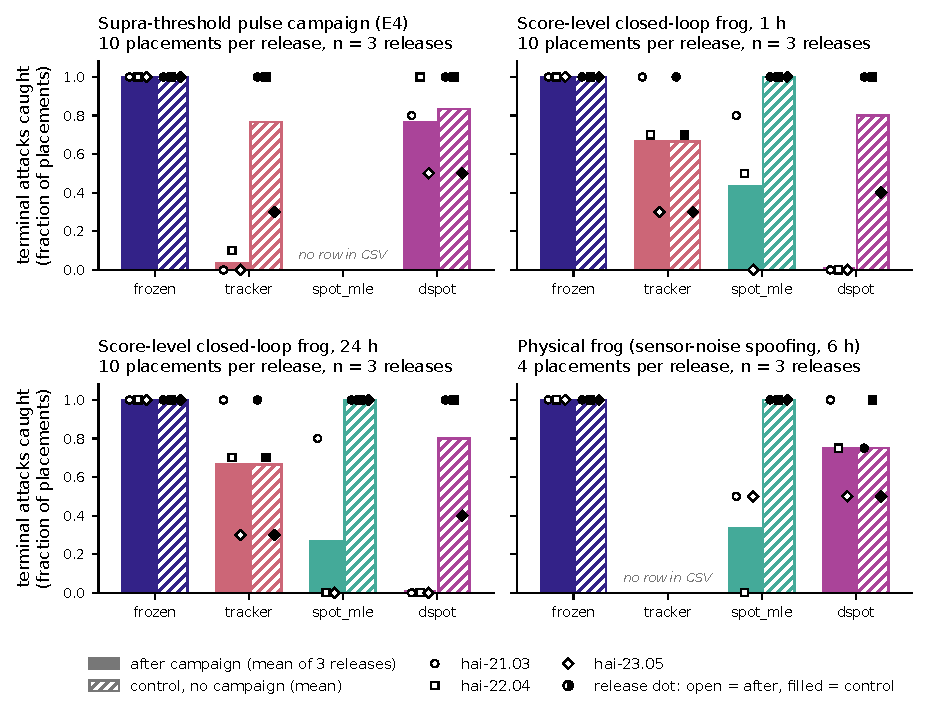
\includegraphics[width=\columnwidth]{figures/fig5_attack_campaigns.pdf}
\caption{Terminal attacks caught after each campaign (solid) and in the matching control (hatched),
for frozen, tracker, spot\_mle and dspot. Each bar is the mean over the three spent HAI releases;
dots are the per-release values, and every release had the same number of placements, so the mean
equals the pooled fraction. Panels: the supra-threshold pulse campaign (E4, 10 placements per
release); the score-level closed-loop frog at 1\,h and 24\,h (10 placements); and the physical frog,
which spoofs noise on three sensors for 6\,h (4 placements). Data status: all four panels are
\textbf{exploratory} results on the normal data of the spent releases. The source CSV has no
spot\_mle row for E4 and no tracker row for the physical frog; both slots are left empty and
labelled.}
\label{fig:campaigns}
\end{figure}

\subsection{Silent poisoning: the closed-loop frog}
\label{sec:frog}

Score-level attacker A2, normal data of the spent releases, 10 placements each: the attacker holds
the score at $0.97\,\tau_t$, then, after a one-hour lead, a 600\,s bump at $1.05\,\tau_0$ follows
(600\,s is the terminal length of every development campaign).

\begin{table*}[t]
\caption{Terminal attacks caught after a closed-loop frog campaign, 30 placements. Data status:
\textbf{exploratory} (normal data of the spent releases).}
\label{tab:frog}
\begin{tabular}{@{}lllll@{}}
\toprule
Rule & 24\,h campaign & 6\,h & 1\,h & open loop, fixed level, 24\,h \\
\midrule
frozen, tracker\_slow, tighten-only & as control & as control & as control & as control \\
tracker & as control & as control & as control & 16/30 (control 20/30) \\
SPOT (moments) & 0/30 & 0/30 & 0/30 & not moved; alarms throughout \\
DSPOT & 0/30 & 0/30 & 0/30 & not moved; alarms throughout \\
SPOT (MLE, refit every 2048 peaks) & 8/30 & 8/30 & 13/30 & 11/30 \\
\bottomrule
\end{tabular}
\end{table*}

Each rule is compared with its own control (the same bump without a campaign). The frozen and both
SPOT controls caught 30/30 and DSPOT's 24/30; the tracker and daily controls already missed some
bumps on the drifting releases, and the campaign did not lower them further. After 1\,h the moments
SPOT threshold stood at 1.1 to 4.5 $\tau_0$; after 24\,h it had grown by more than five orders of
magnitude, and the MLE fit left the floating-point range on one release. A synthetic control with a
light tail (the 60-step moving average of $|N(0, 1)|$, five seeds) did not run away: the moments SPOT
threshold stayed at 0.95 to 0.97 $\tau_0$ and caught every terminal bump, and maximum-likelihood SPOT
rose only to 1.02 to 1.04 $\tau_0$. The runaway therefore depends on the heavy tail of real residual
scores.

\paragraph{A physically realizable version}
The score-level attacker sets the score directly. We also gave the attacker only the readings of
three sensors coupled to one setpoint channel. Every 5 minutes it reads the rule's threshold and
spoofs the largest zero-mean noise whose D1 score, computed by the real world model on the spoofed
history, stays at 0.97 of that threshold; after 6\,h it stops, and 1\,h later the just-detectable
setpoint step follows. This attacker is white-box: it can run the monitor.

\begin{table}[t]
\caption{The physically realizable frog. Data status: \textbf{exploratory} (normal data of the spent
releases).}
\label{tab:physfrog}
\small
\begin{tabular}{@{}p{0.20\columnwidth}p{0.30\columnwidth}p{0.33\columnwidth}@{}}
\toprule
Rule & Terminal caught after campaign / in control (12 placements) & Threshold at the terminal step (median per release) \\
\midrule
frozen & 12 / 12 & 1.0 $\tau_0$ \\
SPOT (MLE) & 4 / 12 & 1.04 to 1.59 $\tau_0$ \\
SPOT (moments) & 6 / 12 & 0.78 to 1.42 $\tau_0$ \\
DSPOT & 9 / 9 & 0.88 to 1.12 $\tau_0$ \\
\bottomrule
\end{tabular}
\end{table}

Controls caught 12 of 12 for frozen and both SPOT variants and 9 of 12 for DSPOT. On HAI 22.04 both
SPOT variants missed the terminal step on all four placements, and the campaign raised no alarm. The
spoofed noise had a scale of 0.02 to 0.04 robust units against frozen and the SPOT variants, and 0.05
to 0.12 against DSPOT, whose moving mean follows the noise-driven rise, so the attacker's cap rises
with the mean rather than with the tail.

\subsection{Registered replication on BATADAL}
\label{sec:batadal}

We registered a second study (tt1b) to test the exploratory findings of Sections~\ref{sec:evt}
and~\ref{sec:frog} on data no analysis here had opened: the C-Town network of
BATADAL~\cite{taormina2018batadal}, whose original attacks conceal themselves in the SCADA readings,
in the re-simulation without that concealment published with the artifact of Erba
et al.~\cite{erba2020concealment}, put on a 15-minute grid. All time-scale settings were fixed in
physical time before access: 1\,h smoothing, episodes merged across 1\,h, one false-alarm episode per
week, a one-day DSPOT mean. The test files hold 14 attacks in 260 days.

\begin{table*}[t]
\caption{Registered hypotheses of tt1b on BATADAL. Data status: \textbf{registered}.}
\label{tab:tt1b}
\begin{tabular}{@{}p{0.07\textwidth}p{0.48\textwidth}p{0.37\textwidth}@{}}
\toprule
Hypothesis & Registered test & Result \\
\midrule
H1 & recall(tracker) $-$ recall(frozen), interval upper bound below 0 & 6/14 vs 14/14, $-0.57$ $[-0.79, -0.29]$: pass \\
H2 & recall(MLE SPOT) $-$ recall(frozen), lower bound at least $-\max(0.10, 2/N)$ & 14/14, difference 0: pass \\
H3 & 24\,h closed-loop frog: DSPOT at least 0.5 below its control; frozen and tighten-only within 0.1 & DSPOT already 0/10 in the control: fail \\
Primary rule & H1 and H2 and H3 & fail \\
\bottomrule
\end{tabular}
\end{table*}

We retain the primary rule as registered and report H3 as uninformative rather than refuted. SWaT and
WADI are registered under the same protocol and were requested on 2026-10-23; they run once their
loaders are added by amendment, and the replication claim is the set of per-dataset outcomes.

H3 failed because real attacks had already blinded DSPOT: its threshold stood 24 times above $\tau_0$
at attack onsets, and it detected 6 of 14 attacks. BATADAL attacks last days, and the smoothed score
spends long stretches in the band below the alarm level, which is exactly where moments SPOT and
DSPOT learn.

\begin{table}[t]
\caption{BATADAL, D1 score. Data status: \textbf{registered} (tt1b).}
\label{tab:batadal}
\begin{tabular}{@{}lccc@{}}
\toprule
Rule (D1) & Recall & False alarms ($\times$ budget) & Onset inflation \\
\midrule
frozen & 14/14 & 0.70 & 1.0 \\
tighten-only & 14/14 & 2.43 & 1.0 \\
SPOT (MLE) & 14/14 & 0.81 & 1.0 \\
daily & 14/14 & 6.34 & 0.69 \\
tracker & 6/14 & 1.83 & 409 \\
tracker\_slow & 5/14 & 0.70 & 74 \\
SPOT (moments) & 6/14 & 0.13 & 26 \\
DSPOT & 6/14 & 0.13 & 24 \\
margin & 3/14 & 0.05 & 173 \\
\bottomrule
\end{tabular}
\end{table}

\begin{figure}[t]
\centering
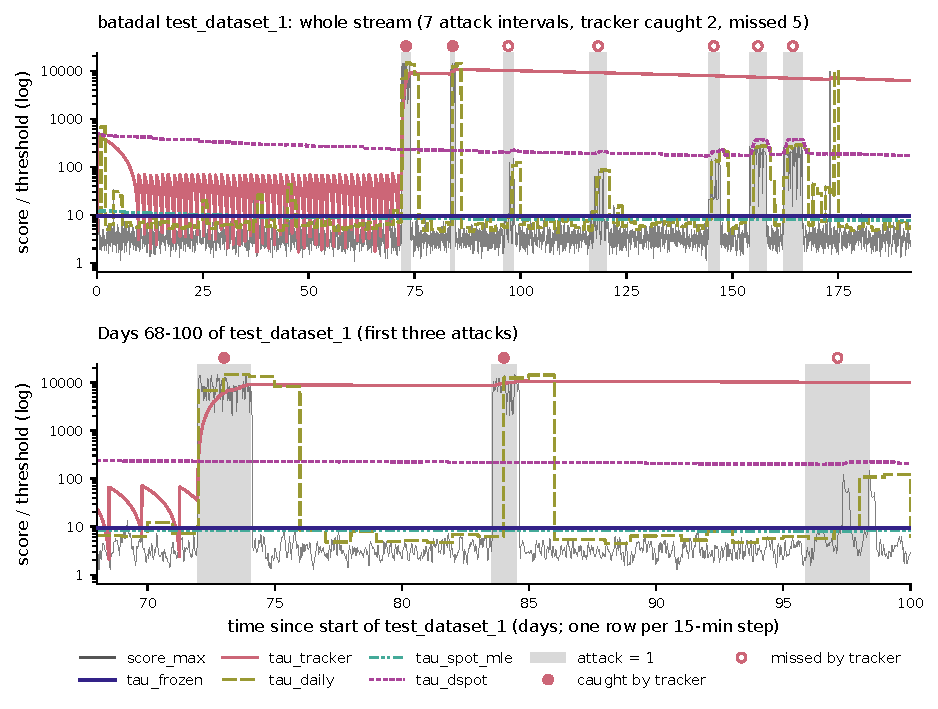
\includegraphics[width=\columnwidth]{figures/fig3_trajectories_batadal.pdf}
\caption{Threshold trajectories on the BATADAL test\_dataset\_1 stream (18,433 steps of 15 minutes,
192 days); layout as in Figure~\ref{fig:hai}. test\_dataset\_1 holds 7 of the 14 attacks; the tracker
caught 2. The lower panel zooms to days 68 to 100, which cover the first three attacks, because the
first attack starts on day 72. score\_max is missing for the first 10 steps ($t = 0$ to 9, 2.5\,h);
those steps are left as a gap and the thresholds are drawn there as given. The days-long attacks lift
the tracker to about $10^4$ and keep DSPOT's threshold far above $\tau_0$ (9.39), while frozen and
spot\_mle stay near $\tau_0$. Data status: \textbf{post-hoc analysis} of the tt1b dataset, which was
opened once for the registered study; the recomputed $\tau_0$ equals the registered value exactly.
Over both test files the traces give frozen 14/14, tracker 6/14, spot\_mle 14/14 and dspot 6/14, the
registered tt1b counts. test\_dataset\_2 is not drawn.}
\label{fig:batadal}
\end{figure}

With the model-free D0 score, MLE SPOT also lost recall (9/14, $[-0.64, -0.14]$). The margin and the
tracker step are scaled by the calibration spread (99.9th percentile minus median); BATADAL's
residual scores are heavy-tailed, so the margin sat 173 times above $\tau_0$. Parameters scaled by a
tail spread are fragile when the tail is heavy.

\section{Design guidance}
\label{sec:design}

A threshold rule's learning region is its attack surface. Every automatic loosening path we tested
could be pushed upward: exceedance tracking and daily recalibration by real attacks and by loud
pulses; tail refitting and moving-mean drift tracking by a closed-loop attacker; the spread and shift
permits by pulses and by benign drift. The rules that held were the ones that never loosen
themselves: frozen, and tighten-only without a permit or with an operator-gated one. A static margin
never loosens either, but it is not safe by construction: on BATADAL its spread-scaled offset sat 173
times above $\tau_0$ and it caught 3 of 14 attacks, the largest recall loss we measured.

We therefore recommend:

\begin{enumerate}
\item \textbf{Let thresholds tighten automatically, never loosen.} A tracker capped at the calibrated
  threshold keeps the frozen threshold's recall on every dataset here and can only add sensitivity in
  quiet periods.
\item \textbf{Route loosening through an operator} who confirms the plant is in normal operation, and
  treat a request to loosen during or soon after an alarm as suspect.
\item \textbf{Recalibrate offline on verified clean data}, as a change-controlled event, when drift
  raises false alarms; our frozen thresholds held 0.66 to 2.23 episodes per day on four HAI test
  periods.
\item \textbf{Watch the threshold.} Log $\tau_t$; a threshold that rises during an incident, or climbs
  steadily without alarms, is itself an indicator.
\end{enumerate}

The cost is false alarms under benign upward drift: on a development split of HAI 23.05 the
tighten-only rule ran at 5.98 times the budget against 4.05 for the frozen threshold. A static margin
can cut that cost on some plants (HAI 23.05 development: 0.58 times the budget) but costs recall on
others (voraus-AD: 12 points; BATADAL: 11 of 14 attacks), and should not be used where the
calibration spread is set by a heavy tail.

\section{Limitations}
\label{sec:limitations}

\begin{itemize}
\item Two registered studies with one primary dataset each; HAI 20.07 shares a testbed with the
  development releases, and BATADAL has 14 attacks.
\item HyGrid-ICS is a single simulated day with 2.5\,h of unlabelled final time; voraus-AD anomalies
  are not attacks. Post-hoc, 0.15\% of HyGrid-ICS's label-blind development rows (251 short runs)
  carry an attack label, against 83\% of its final rows, so its calibration is very slightly
  contaminated.
\item The pulse campaigns and both frogs are synthetic. The score-level frog sets the score directly
  and reads $\tau_t$; the physically realizable version also runs the monitor itself on the spoofed
  history to choose each noise scale. Both are white-box upper bounds.
\item SPOT's behaviour depends on the tail estimator and on the score's tail shape; we report both.
\item Parameters scaled by a calibration spread (the static margin and the tracker step) are fragile
  on heavy-tailed scores: on BATADAL the margin sat 173 times above $\tau_0$ and missed 11 of 14
  attacks.
\item Event recall counts any alarm inside a labelled interval; we do not model operator response
  time.
\item Our monitor is one world-model residual and one model-free score; reconstruction-based
  detectors were not tested.
\item No claim of runtime authority, deployment safety or incident prevention follows from these
  results.
\end{itemize}

\section{Conclusion}

On four never-opened datasets, adaptive thresholds that learn from exceedances missed attacks that a
frozen threshold caught, because earlier attacks had raised them. Extreme-value thresholds avoided
that failure on the HAI data but not on days-long BATADAL attacks, and an attacker who stayed under
them could drive them upward without an alarm. A threshold that only tightened itself matched the
frozen threshold's recall on all seven datasets we examined.

\bibliographystyle{plain}
\bibliography{refs}

\appendix

\section*{Open science}

The two pre-registrations, the data-access ledger, the attack and threshold harnesses, the
registered-gate verifiers and the figure data and plotting code are available in the anonymized
artifact at \url{https://anonymous.4open.science/...}, which also contains the result files behind
every number in this paper and the verifier reports (27 of 27 checks for tt1, 8 of 8 for tt1b).
% TODO: replace with the anonymous.4open.science URL of the anonymized artifact before submission;
% the de-anonymized repository and the artifact DOI are added in the camera-ready version.
The raw datasets are not redistributed here and are available from their publishers: HAI from its
dataset repository, BATADAL from Taormina et al.~\cite{taormina2018batadal} and the no-concealment
re-simulation from the artifact of Erba et al.~\cite{erba2020concealment}, voraus-AD from Brockmann
et al.~\cite{brockmann2024voraus}, and HyGrid-ICS from its Zenodo record~\cite{yolcu2026hygrid}.
Reproducing the registered results requires one access to each raw dataset under the access rules
recorded in the ledger.

\end{document}
